\section{Introduction to Fourier coefficients}
\label{sec:fouriercoeffintro}

\subsection*{Resources}
\begin{itemize}
    \item Book: 1.4 (\url{https://see.stanford.edu/materials/lsoftaee261/book-fall-07.pdf})
    \item Video: Lecture 2 (\url{https://www.youtube.com/watch?v=1rqJl7Rs6ps})
\end{itemize}

\subsection*{Challenge}
Deduce in a simple way the Fourier coefficients $a_1$ and $b_1$ in the Fourier series
\begin{equation}
    \sum_{k=1}^{N} a_k cos(2 \pi k t) + b_k sin(2 \pi k t)
\end{equation}

for a signal made up of multiple sine signals
\begin{equation}
    \sum_{k=1}^{N} A_k sin(2 \pi k t + \phi_k)
\end{equation}

for the following cases:
\begin{enumerate}
    \item $N=1$, $k=1$, $A_1=1$, $\phi_1=0$
    \item $N=1$, $k=1$, $A_1=1$, $\phi_1=\pi/2$
    \item $N=1$, $k=1$, $A_1=1$, $\phi_1=\pi/5$
\end{enumerate}

Hint: Using $sin(A+B) = sin(A) cos(B) + cos(A) sin(B)$ it should is possible to find the answer without resorting to complex calculation.

\subsection*{Solutions}
\begin{enumerate}
    \item MD5(o\_$a_k$) = a2c1fe\ldots, MD5(p\_$b_k$) = de80c6\ldots
    \item MD5(a\_$a_k$) = 718a6c\ldots, MD5(s\_$b_k$) = f86f0c\ldots
    \item MD5(d\_$a_k$) = 93d647\ldots, MD5(f\_$b_k$) = 9a7b58\ldots
\end{enumerate}

\timebox




%%%%%%%%%%%%%%%%%%%%%%%%%%%%%%%%%
\newpage
%%%%%%%%%%%%%%%%%%%%%%%%%%%%%%%%%

\section{Even and odd functions}

\subsection*{Resources}
\begin{itemize}
    \item Wikipedia: \url{https://en.wikipedia.org/wiki/Even_and_odd_functions}
\end{itemize}

\subsection*{Challenge}
Referring in part to the cases in challenge \ref{sec:fouriercoeffintro}, sum the points of all the following TRUE statements:

1 point: Case 1 is an odd function

2 points: Case 1 is an even function

4 points: Case 2 is an odd function

8 points: Case 2 is an even function

16 point: Case 3 is an odd function

32 points: Case 3 is an even function

64 points: $f(x)=Sin(x)$ is an odd function

128 points: $f(x)=Sin(x)$ is an even function

256 points: $f(x)=Cos(x)$ is an odd function

512 points: $f(x)=Cos(x)$ is an even function

1024 points: $f(x)=x$ is an odd function

2048 points: $f(x)=x$ is an even function

\subsection*{Solution}
X

\hash{g}{6a18c0}

\timebox




%%%%%%%%%%%%%%%%%%%%%%%%%%%%%%%%%
\newpage
%%%%%%%%%%%%%%%%%%%%%%%%%%%%%%%%%

\section{Fourier Coefficients of sin(x)}
\label{sec:fcsinx}

\subsection*{Resources}
\begin{itemize}
    \item Book: 1.4 (\url{https://see.stanford.edu/materials/lsoftaee261/book-fall-07.pdf})
    \item Video: Lecture 2 (\url{https://www.youtube.com/watch?v=1rqJl7Rs6ps})
\end{itemize}

\subsection*{Comments}
You should be able to follow the derivation of the formula for Fourier coefficients ($C_k$'s) in the video. Feel free to seek help if you have trouble.

\subsection*{Challenge}
By writing $sin(x)$ in exponential form, deduce the Fourier coefficients ($C_k$'s) for the function $sin(x)$, for the following cases:
\begin{enumerate}
    \item k = -1
    \item k = 0
    \item k = 1
\end{enumerate}

\subsection*{Solutions}
\subsubsection{k=-1}
X

\hash{h}{28f251}

\subsubsection{k=0}
X

\hash{j}{4fd3f6}

\subsubsection{k=1}
X

\hash{k}{e82a2a}

\timebox




%%%%%%%%%%%%%%%%%%%%%%%%%%%%%%%%%
\newpage
%%%%%%%%%%%%%%%%%%%%%%%%%%%%%%%%%

\section{Fourier Coefficients of 1 + sin(x)}

\subsection*{Resources}
\begin{itemize}
    \item Book: 1.4 (\url{https://see.stanford.edu/materials/lsoftaee261/book-fall-07.pdf})
    \item Video: Lecture 2 (\url{https://www.youtube.com/watch?v=1rqJl7Rs6ps})
\end{itemize}

\subsection*{Comments}
You should be able to follow the derivation of the formula for Fourier coefficients in the video. Feel free to seek help if you have trouble.

\subsection*{Challenge}
Continuing from challenge \ref{sec:fcsinx}, deduce the Fourier coefficients ($C_k$'s) for the function $1+sin(x)$, for the following cases:
\begin{enumerate}
    \item k = -1
    \item k = 0
    \item k = 1
\end{enumerate}

\subsection*{Solutions}
\subsubsection{k=-1}
X

\hash{z}{39e026}

\subsubsection{k=0}
X

\hash{x}{0ef183}

\subsubsection{k=1}
X

\hash{c}{fda796}

\timebox




%%%%%%%%%%%%%%%%%%%%%%%%%%%%%%%%%
\newpage
%%%%%%%%%%%%%%%%%%%%%%%%%%%%%%%%%

\section{Relation of positive and negative Fourier coefficients for a real signal}

\subsection*{Resources}
\begin{itemize}
    \item Book: 1.4 (\url{https://see.stanford.edu/materials/lsoftaee261/book-fall-07.pdf})
    \item Video: Lecture 2 (\url{https://www.youtube.com/watch?v=1rqJl7Rs6ps})
\end{itemize}

\subsection*{Challenge}
If the Fourier coefficient $C_1$ is $4 + 6i$, what is the Fourier coefficient $C_{-1}$?

\subsection*{Solution}
X

\hash{m}{36ab38}

\timebox




%%%%%%%%%%%%%%%%%%%%%%%%%%%%%%%%%
\newpage
%%%%%%%%%%%%%%%%%%%%%%%%%%%%%%%%%

\section{Converting between trigonometric and exponential forms}
\label{sec:trigexpconvert}

\subsection*{Resources}
\begin{itemize}
    \item Book: 1.4 (\url{https://see.stanford.edu/materials/lsoftaee261/book-fall-07.pdf})
    \item Video: Lecture 2 (\url{https://www.youtube.com/watch?v=1rqJl7Rs6ps})
\end{itemize}

\subsection*{Challenge}
Derive an expression for $C_k$ in terms of the $a_k$'s and $b_k$'s in the expression
\begin{equation}
    f(t) = \frac{a_0}{2} + \sum_{k=1}^{k=N} a_k cos(2 \pi k t) + b_k sin(2 \pi k t) = \sum_{k=-N}^{k=N} C_k e^{2 \pi i k t}
\end{equation}

To check your answer, substitute $a_0 = 1$, $a_1 = 3$ and $b_1 = 5$ as required to calculate $C_k$ for k = -1, 0 and 1.

\subsection*{Solutions}
\subsubsection{k=-1}
X

\hash{v}{052df3}

\subsubsection{k=0}
X

\hash{b}{fb29ff}

\subsubsection{k=1}
X

\hash{n}{284b53}

\timebox




%%%%%%%%%%%%%%%%%%%%%%%%%%%%%%%%%
\newpage
%%%%%%%%%%%%%%%%%%%%%%%%%%%%%%%%%

\section{The Fourier series of $f(t)=t$: $C_0$}

\subsection*{Resources}
\begin{itemize}
    \item Book: 1.5, 1.7 (\url{https://see.stanford.edu/materials/lsoftaee261/book-fall-07.pdf})
    \item Video: Lecture 3 (\url{https://www.youtube.com/watch?v=BjBb5IlrNsQ})
\end{itemize}

\subsection*{Challenge}
Considering the function $f(t)=t$ over the interval 0 to 1, calculate the Fourier coefficient $C_0$ using the derived formula for Fourier coefficients. Compare with the average over the interval.

\subsection*{Solution}
X

\hash{aa}{2708ad}

\timebox




%%%%%%%%%%%%%%%%%%%%%%%%%%%%%%%%%
\newpage
%%%%%%%%%%%%%%%%%%%%%%%%%%%%%%%%%

\section{The Fourier series of $f(t)=t$: $C_k$}

\subsection*{Resources}
\begin{itemize}
    \item Book: 1.5, 1.7 (\url{https://see.stanford.edu/materials/lsoftaee261/book-fall-07.pdf})
    \item Video: Lecture 3 (\url{https://www.youtube.com/watch?v=BjBb5IlrNsQ})
\end{itemize}

\subsection*{Challenge}
Considering the function $f(t)=t$, calculate a general expression for the Fourier coefficients $C_k$ where $k \ne 0$.

To check your answer, evaluate the Fourier coefficient for $k=-30$.

\subsection*{Solution}
X

\hash{bb}{e904e9}

\timebox




%%%%%%%%%%%%%%%%%%%%%%%%%%%%%%%%%
\newpage
%%%%%%%%%%%%%%%%%%%%%%%%%%%%%%%%%

\section{The Fourier series of $f(t)=t$ in exponential form}
\label{sec:fstexpform}

\subsection*{Resources}
\begin{itemize}
    \item Book: 1.4 (\url{https://see.stanford.edu/materials/lsoftaee261/book-fall-07.pdf})
    \item Video: Lecture 3 (\url{https://www.youtube.com/watch?v=BjBb5IlrNsQ})
\end{itemize}

\subsection*{Challenge}
Write the function $f(t)=t$ in terms of its infinite exponential Fourier series.

To check your answer, evaluate the Fourier series up to $n=2$ with $t=0.8$.

The graph with increasing values of $n$ looks like this:

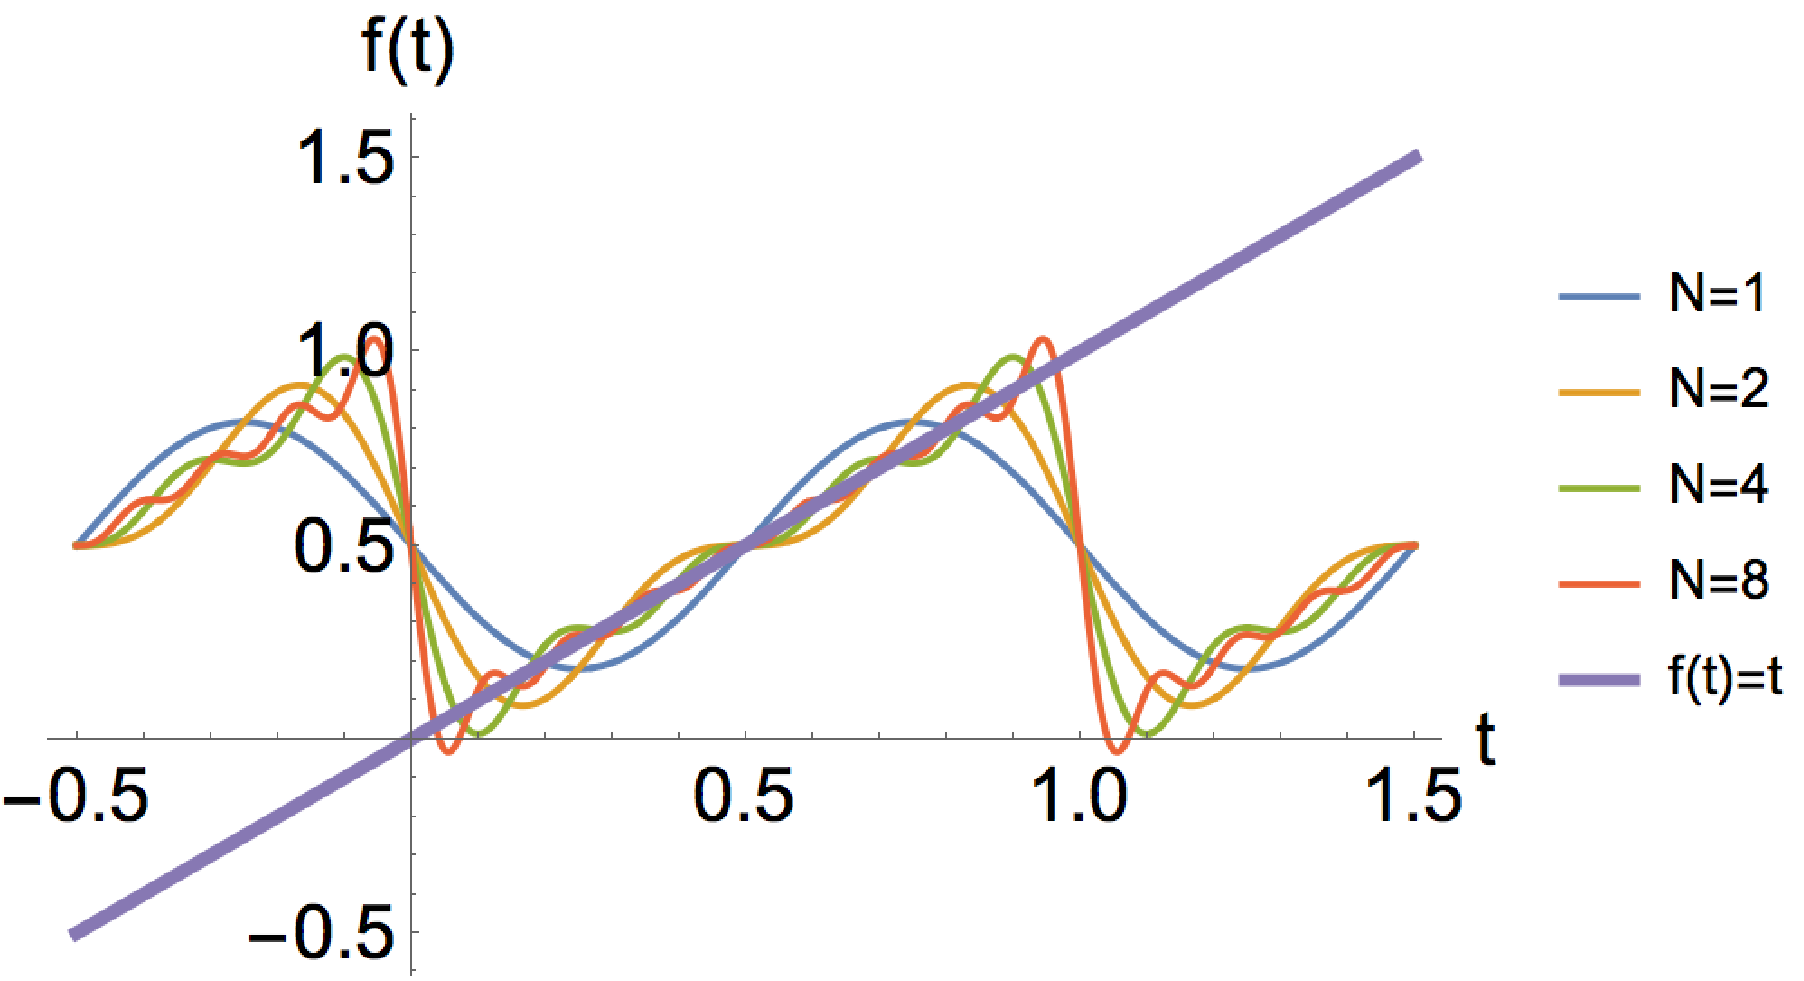
\includegraphics{fourier_series_t.png}

\subsection*{Solution}
X

\hash{cc}{d21e19}

\timebox




%%%%%%%%%%%%%%%%%%%%%%%%%%%%%%%%%
\newpage
%%%%%%%%%%%%%%%%%%%%%%%%%%%%%%%%%

\section{The Fourier series of $f(t)=t$ in trigonometric form}

\subsection*{Resources}
\begin{itemize}
    \item Book: 1.5, 1.7 (\url{https://see.stanford.edu/materials/lsoftaee261/book-fall-07.pdf})
    \item Video: Lecture 2 (\url{https://www.youtube.com/watch?v=1rqJl7Rs6ps})
\end{itemize}

\subsection*{Comment}
Many textbooks will work in terms of ``Fourier sine series'' and ``Fourier cosine series''. For a function that is perfectly even or odd, it is possible to write a Fourier series using one of these two forms. There are direct approaches to calculating sine and cosine Fourier series, in contrast to the route taken here via the exponential form. We will continue to work in the exponential form however, since not only does this provide a deeper understanding, but you can always easily switch between exponential and trigonometric forms if you really want to.


\subsection*{Challenge}
Re-write the series obtained in challenge \ref{sec:fstexpform} in terms of a trigonometric infinite series (ie, using sines and cosines).

To check your answer, evaluate the Fourier series up to $n=2$ with $t=0.8$ and ensure that you get the same answer as you did for challenge \ref{sec:fstexpform}.

\timebox




%%%%%%%%%%%%%%%%%%%%%%%%%%%%%%%%%
\newpage
%%%%%%%%%%%%%%%%%%%%%%%%%%%%%%%%%
\section{Periods other than unity}

\subsection*{Resources}
\begin{itemize}
    \item Book: 1.6 (\url{https://see.stanford.edu/materials/lsoftaee261/book-fall-07.pdf})
\end{itemize}

\subsection*{Challenge}
Determine the Fourier series for the same function as in \ref{sec:fstexpform} ($f(t)=t$), except approximate the function over the region $1<x<3$ instead of $0<x<1$.

To check your answer, evaluate the Fourier series up to $n=2$ with $t=1.8$.

The graph with increasing values of $n$ looks like this:

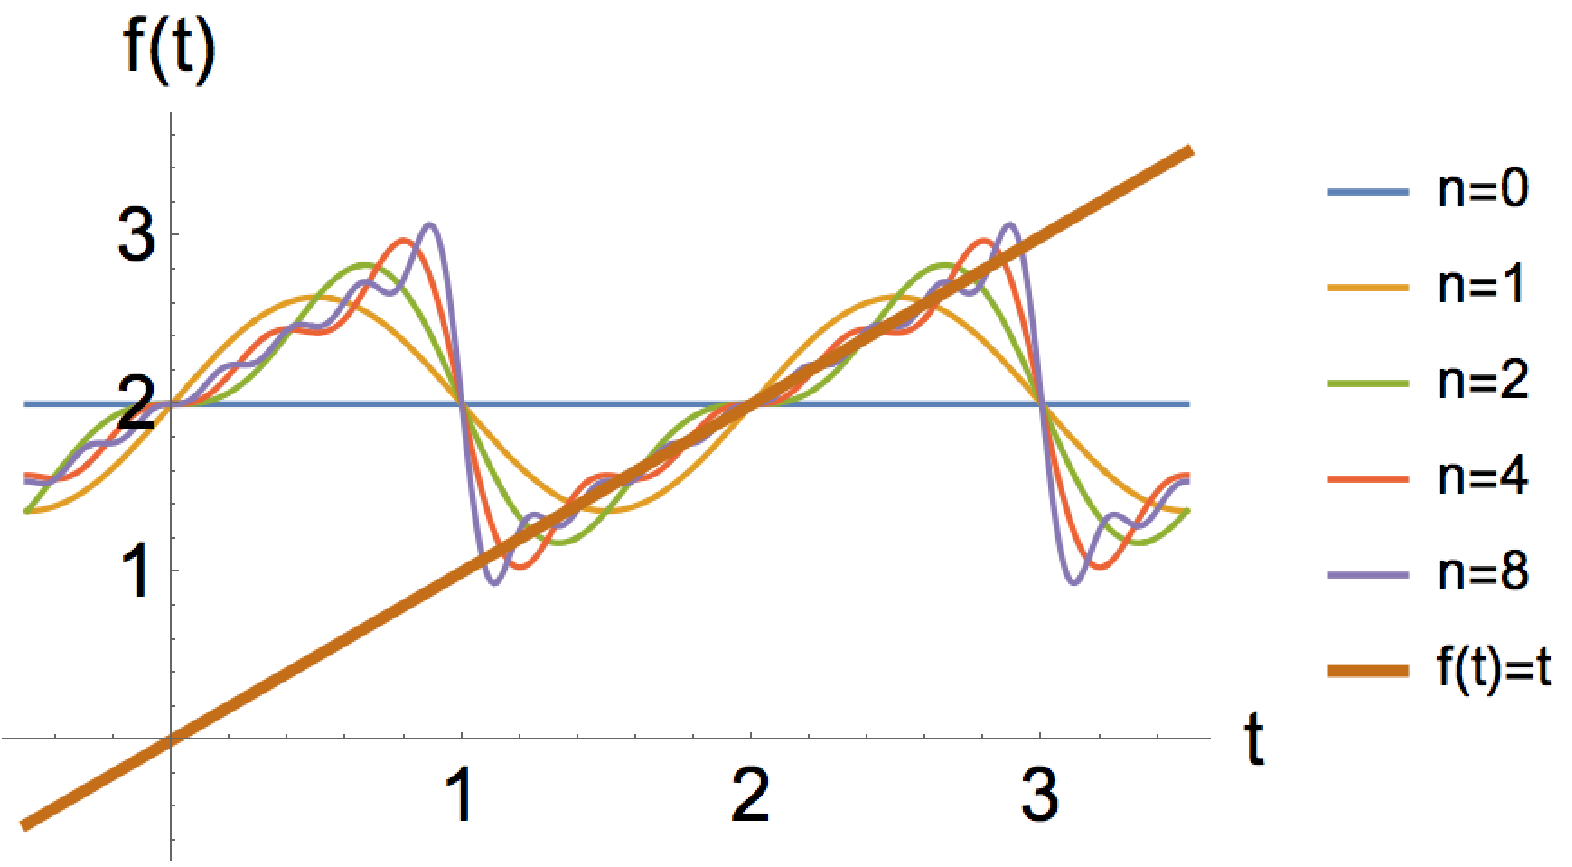
\includegraphics{fs_other_periods.png}

\subsection*{Solution}
X

\hash{dd}{83e943}

\timebox




%%%%%%%%%%%%%%%%%%%%%%%%%%%%%%%%%
\newpage
%%%%%%%%%%%%%%%%%%%%%%%%%%%%%%%%%
\section{Infinite series}

\subsection*{Comment}
It is important to understand why some series are infinite, while others are not (well, technically all series are infinite since they all involve sums to $n=\infty$, however for some series the Fourier coefficients are all zero above a certain value of $n$). Therefore, make sure you understand why the answer is as it is, below. If you don't, be sure to discuss with others.

\subsection*{Challenge}
The Fourier series is a sum to $\pm \infty$, however in some cases the coefficients ($C_k$'s) are zero beyond a certain number of terms. Which of the terms below will have Fourier coefficients that are all zero after a certain number of terms? Sum the points of these functions.

1 point: $x$

2 points: $x^2$

4 points: $cos(2 x) + 3 sin(7 x)$

8 points: $e^{2 \pi i x}$

\subsection*{Solution}
X

\hash{ee}{8e05a4}

\timebox




%%%%%%%%%%%%%%%%%%%%%%%%%%%%%%%%%
\newpage
%%%%%%%%%%%%%%%%%%%%%%%%%%%%%%%%%
\section{k-symmetry}

\subsection*{Challenge}
Determine what X and Y represent algebraically.
\begin{equation}
    cos(k \pi t) = \frac{1}{2} e^{-k i\pi t} + \frac{1}{2} e^{\bm{X} i \pi x}
\end{equation}
\begin{equation}
    sin(k \pi t) = \frac{1}{2} i e^{\bm{Y} i \pi t} - \frac{1}{2} i e^{k i \pi t}
\end{equation}

To check your answers you may substitute any appropriate values from the following list: $k=2$, $t=1$

\subsection*{Solution}
X

\hash{ff}{942d6f}

Y

MD5(gg\_Y) = a379b8\ldots

\timebox




%%%%%%%%%%%%%%%%%%%%%%%%%%%%%%%%%
\newpage
%%%%%%%%%%%%%%%%%%%%%%%%%%%%%%%%%
\section{Direct trigonometric calculation of a Fourier series: the coefficients}
\label{sec:fs_squarewave}

\section*{Comment}
This challenge introduces several key concepts at once, including decoupling of integral intervals and periodicity, the concept of a square wave and direct trigonometric evaluation of Fourier series. If you can master this you'll be in a really strong position.

It is hopefully clear now that for real signals, due to the symmetry of the positive and negative k's, one can fully compose Fourier series in terms of sine and cosine. In challenge \ref{sec:trigexpconvert} we saw the formula for the function in terms of Fourier coefficients $a_0$, $a_n$ and $b_n$. While we will not use this approach, it is important to be able to utilise such a formulation since this is the way some books present it and some people have learnt it. Therefore, without proof, the coefficients can be calculated using

\begin{equation}
    a_k = \frac{2}{T} \int_{t_0}^{t_0+T} f(t) Cos(2 \pi k t/T)
\end{equation}
\begin{equation}
    b_k = \frac{2}{T} \int_{t_0}^{t_0+T} f(t) Sin(2 \pi k t/T)
\end{equation}

\subsection*{Challenge}
Using the direct trigonometric Fourier series, obtain a general expression for the $a_k$ and $b_k$ coefficients for the square-wave signal with periodicity 4

\begin{equation}
    f(t)=
    \begin{cases}
        1 & \text{for } -1<t<1 \\
        0 & \text{for } 1<t<3
    \end{cases}
\end{equation}

A graph of the function, including the solution for various values of $n$, is shown here:

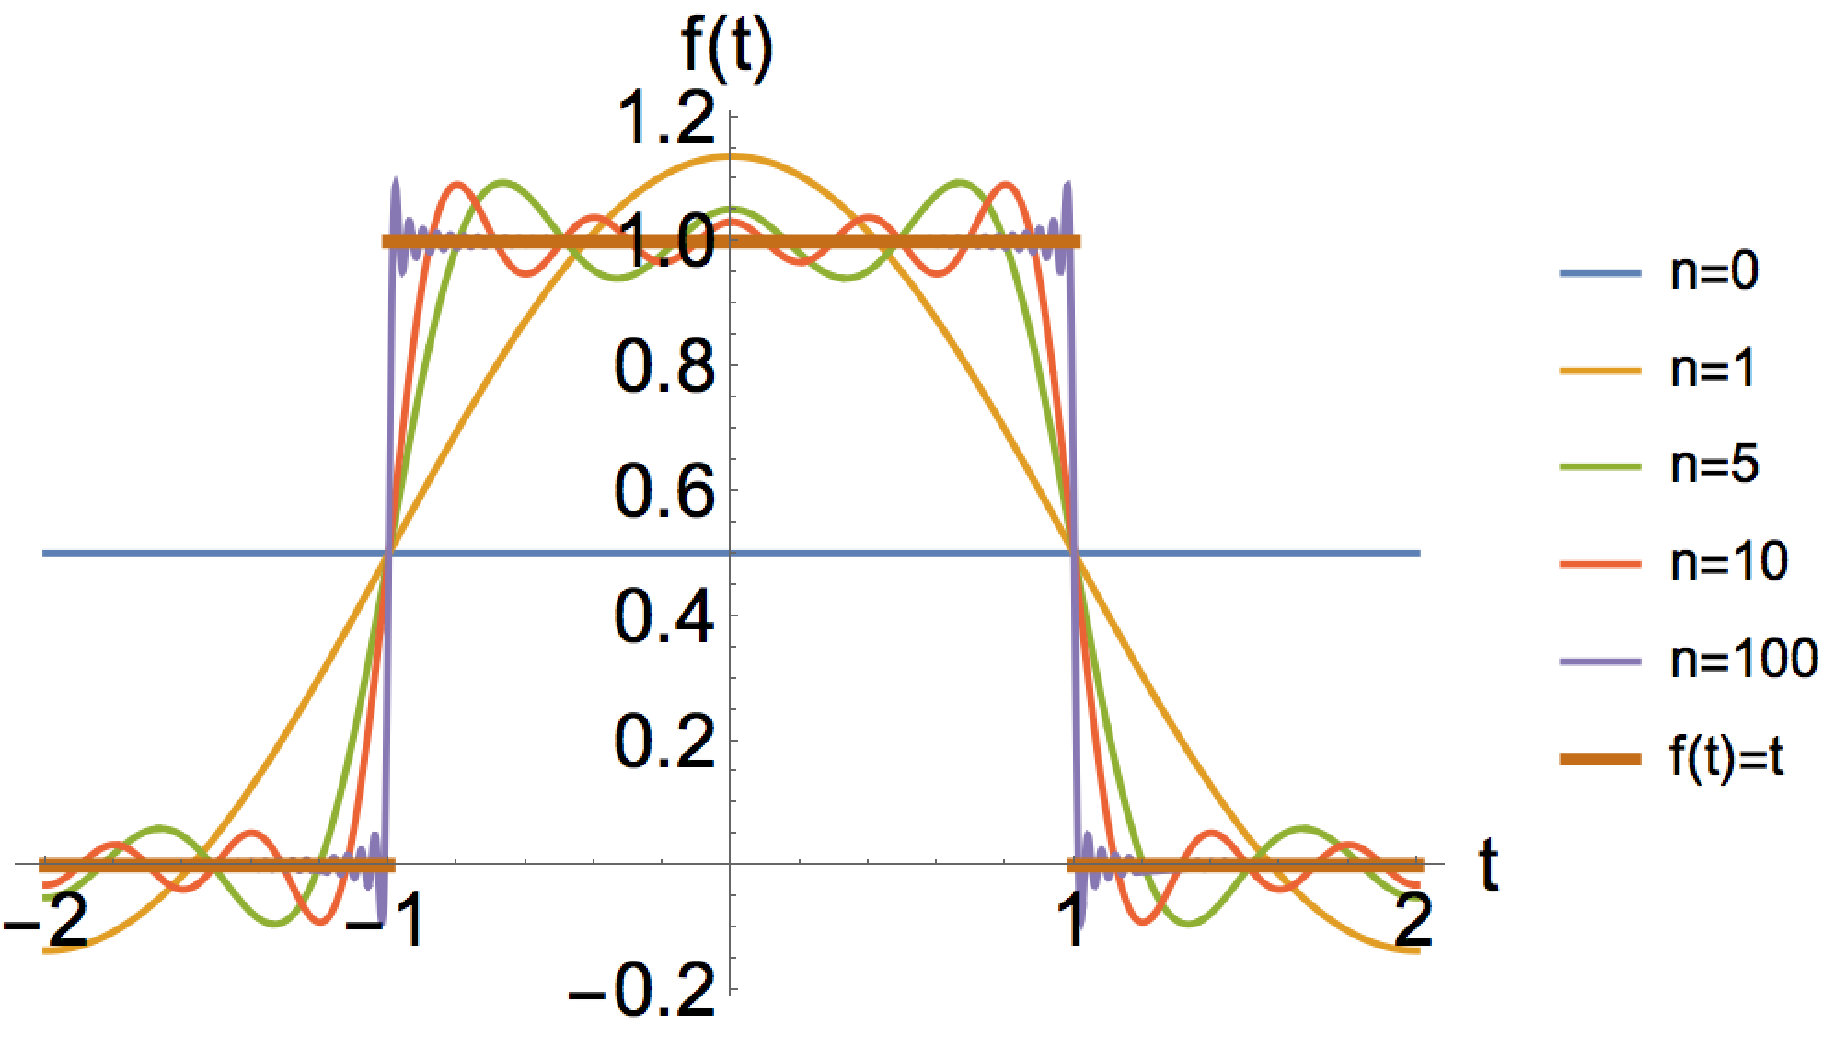
\includegraphics{fs_square_wave.png}

Note the symmetry of the problem. Can you see what terms will be zero? To check your solution, calculate $a_k$ and $b_k$ for $k=0$, $k=2$ and $k=3$. Also note that you will have to break the integrals into two parts and sum them in order to tackle this problem.

\subsection*{Solution}
\begin{tabular}{|l|l|l|}
    \hline
    $k$ & $a_k$ & $b_k$ \\
    \hline
    0 & MD5(hh\_X)=e57c15\ldots & MD5(ii\_X)=377fe2\ldots \\
    2 & MD5(jj\_X)=54aaa1\ldots & MD5(kk\_X)=be063f\ldots \\
    3 & MD5(mm\_X)=b8fce7\ldots & MD5(nn\_X)=b6fbaf\ldots \\
    \hline
\end{tabular}

\timebox




%%%%%%%%%%%%%%%%%%%%%%%%%%%%%%%%%
\newpage
%%%%%%%%%%%%%%%%%%%%%%%%%%%%%%%%%
\section{Direct trigonometric calculation of a Fourier series: the series}

\subsection*{Challenge}
Calculate the Fourier series for the square wave introduced in challenge \ref{sec:fs_squarewave} using direct trigonometric calculation for up to $n=3$. Check your solution by evaluating for $t=0.1$.

\subsection*{Solution}
\six{}

\hash{oo}{bd7e5e}

\timebox




%%%%%%%%%%%%%%%%%%%%%%%%%%%%%%%%%
\newpage
%%%%%%%%%%%%%%%%%%%%%%%%%%%%%%%%%
\section{2D orthogonal vectors}

\subsection*{Resources}
\begin{itemize}
    \item Book: 1.9 (\url{https://see.stanford.edu/materials/lsoftaee261/book-fall-07.pdf})
\end{itemize}

\subsection*{Challenge}
Sum the points of the vectors in 2D that are orthogonal:

1 point: (5, 4) and (-1, 1.25)

2 points:  (2, -3) and (-6, 4)

4 points: (-2.25, 1.5) and (2, 3)

8 points: (4.5, 4) and (3, -3.375)

16 points: (6, 4) and (4, -6)

32 points: (5, 1) and (-2, 8.125)

64 points: (0, 1) and (1, 0)

128 points: (1, 1) and (1, 1)

\subsection*{Solution}
\six{}

\hash{pp}{92843f}

\timebox




%%%%%%%%%%%%%%%%%%%%%%%%%%%%%%%%%
\newpage
%%%%%%%%%%%%%%%%%%%%%%%%%%%%%%%%%
\section{Orthonormal basis}

\subsection*{Resources}
\begin{itemize}
    \item Video: \url{https://www.khanacademy.org/math/linear-algebra/alternate-bases/orthonormal-basis/v/linear-algebra-introduction-to-orthonormal-bases}
\end{itemize}

\subsection*{Challenge}
Sum the points of the following vectors that form an orthonormal basis:

1 point :
($\displaystyle \frac{1}{\sqrt{5}}, \frac{2}{\sqrt{5}}$) and
($\displaystyle \frac{2}{\sqrt{5}}, \frac{4}{\sqrt{5}}$)

2 points:
($\displaystyle \frac{2}{\sqrt{5}}$, $\displaystyle \frac{1}{\sqrt{5}}$) and
($\displaystyle \frac{-1}{\sqrt{5}}$, $\displaystyle \frac{2}{\sqrt{5}}$)

4 points:
($\displaystyle \frac{2}{\sqrt{2}}, \sqrt{\frac{7}{8}}, \frac{1}{\sqrt{6}}$),
($\displaystyle -\sqrt{\frac{2}{5}}, \frac{7}{\sqrt{14}}, -\frac{1}{\sqrt{6}}$) and
($\displaystyle \frac{1}{\sqrt{3}},  \frac{1}{5 \sqrt{3}}, -\frac{7}{5 \sqrt{3}}$)

8 points:
($\displaystyle \frac{1}{\sqrt{21}}, \frac{2}{\sqrt{21}}, \frac{4}{\sqrt{21}}$),
($\displaystyle -\sqrt{\frac{2}{7}}, \frac{3}{\sqrt{14}}, -\frac{1}{\sqrt{14}}$) and
($\displaystyle \sqrt{\frac{2}{3}},  \frac{1}{\sqrt{6}}, -\frac{1}{\sqrt{6}}$)

16 points:
($\displaystyle \frac{1}{\sqrt{6}}, \sqrt{\frac{2}{3}}, \frac{1}{\sqrt{6}}$),
($\displaystyle -\frac{1}{\sqrt{2}},  \frac{2 \sqrt{2}}{5}, -\frac{3}{5 \sqrt{2}}$) and
($\displaystyle \frac{1}{\sqrt{3}},  \frac{1}{5 \sqrt{3}}, -\frac{7}{5 \sqrt{3}}$)

32 points:
($0, 2$) and ($2, 0$)

64 points:
($0, 1$) and ($1, 0$)

\subsection*{Solution}
\six{}

\hash{qq}{097fd7}

\timebox




%%%%%%%%%%%%%%%%%%%%%%%%%%%%%%%%%
\newpage
%%%%%%%%%%%%%%%%%%%%%%%%%%%%%%%%%
\section{Natural basis}

\subsection*{Resources}
\begin{itemize}
    \item Book: 1.9 (\url{https://see.stanford.edu/materials/lsoftaee261/book-fall-07.pdf})
\end{itemize}

\subsection*{Challenge}
Sum the components of the following vectors of an orthonormal basis in $\mathbb{R}^{300}$ space:

\begin{itemize}
    \item First component of the first vector
    \item first component of the second vector
    \item 200th component of the 100th vector
    \item 200th component of the 200th vector
    \item last component of the 299th vector
    \item last component of the last vector
\end{itemize}

\subsection*{Solution}
\six{}

\hash{rr}{095c77}

\timebox




%%%%%%%%%%%%%%%%%%%%%%%%%%%%%%%%%
\newpage
%%%%%%%%%%%%%%%%%%%%%%%%%%%%%%%%%
\section{Orthonormal basis for Fourier series}

\subsection*{Resources}
\begin{itemize}
    \item Book: 1.9 (\url{https://see.stanford.edu/materials/lsoftaee261/book-fall-07.pdf})
\end{itemize}

\subsection*{Comment}
The previous challenges have focussed on the orthogonality and orthonormality of vectors. We now make the jump to functions. As chapter 1.9 explains, although its not perfect, the analogy between vectors and functions is a good way to help understand and visualise the role that the terms of a Fourier series play in defining a basis upon which to describe a function.

\subsection*{Challenge}
Starting from the inner product of two terms ($e^{2 \pi i k_1 t}$, $e^{2 \pi i k_2 t}$) of a Fourier series, demonstrate that the terms of a Fourier series form an orthonormal basis. \textbf{Show a full derivation}.

To check your intuition, you may evaluate the following cases:

$X = (e^{2 \pi i k_1 t}, e^{2 \pi i k_1 t})$

$Y = (e^{2 \pi i k_1 t}, e^{2 \pi i k_2 t})$

\subsection*{Solution}
If you are not confident about your derivation, please check with someone else. If there is any step that you do not fully understand, do not hesitate to ask. If you do not understand the connection between previous challenges on vectors and this challenge using functions, do not hesitate to ask someone.

\textbf{X}

\hash{ss}{8f7f41}

\textbf{Y}

MD5(tt\_Y) = 2c669b\ldots

\timebox




%%%%%%%%%%%%%%%%%%%%%%%%%%%%%%%%%
\newpage
%%%%%%%%%%%%%%%%%%%%%%%%%%%%%%%%%
\section{Circles and Fourier series}

\subsection*{Resources}
\begin{itemize}
    \item Video 1: \url{https://www.youtube.com/watch?v=Y9pYHDSxc7g}
    \item Video 2: \url{https://www.youtube.com/watch?v=LznjC4Lo7lE}
\end{itemize}

\subsection*{Comment}
In the first lecture we saw how it was possible to approximate any function given enough circles. Here we link what you have learned back to that first lecture. I strongly recommend viewing the fun and informative videos listed here under Resources. In summary, by building a Fourier series you are representing a function using an orthonormal basis, where each component of the basis can be considered visually as a circle operating with individual radius and frequency on the real-imaginary plane. If, after completing this challenge, that last sentence makes sense to you, then you have achieved the first major goal of this course.

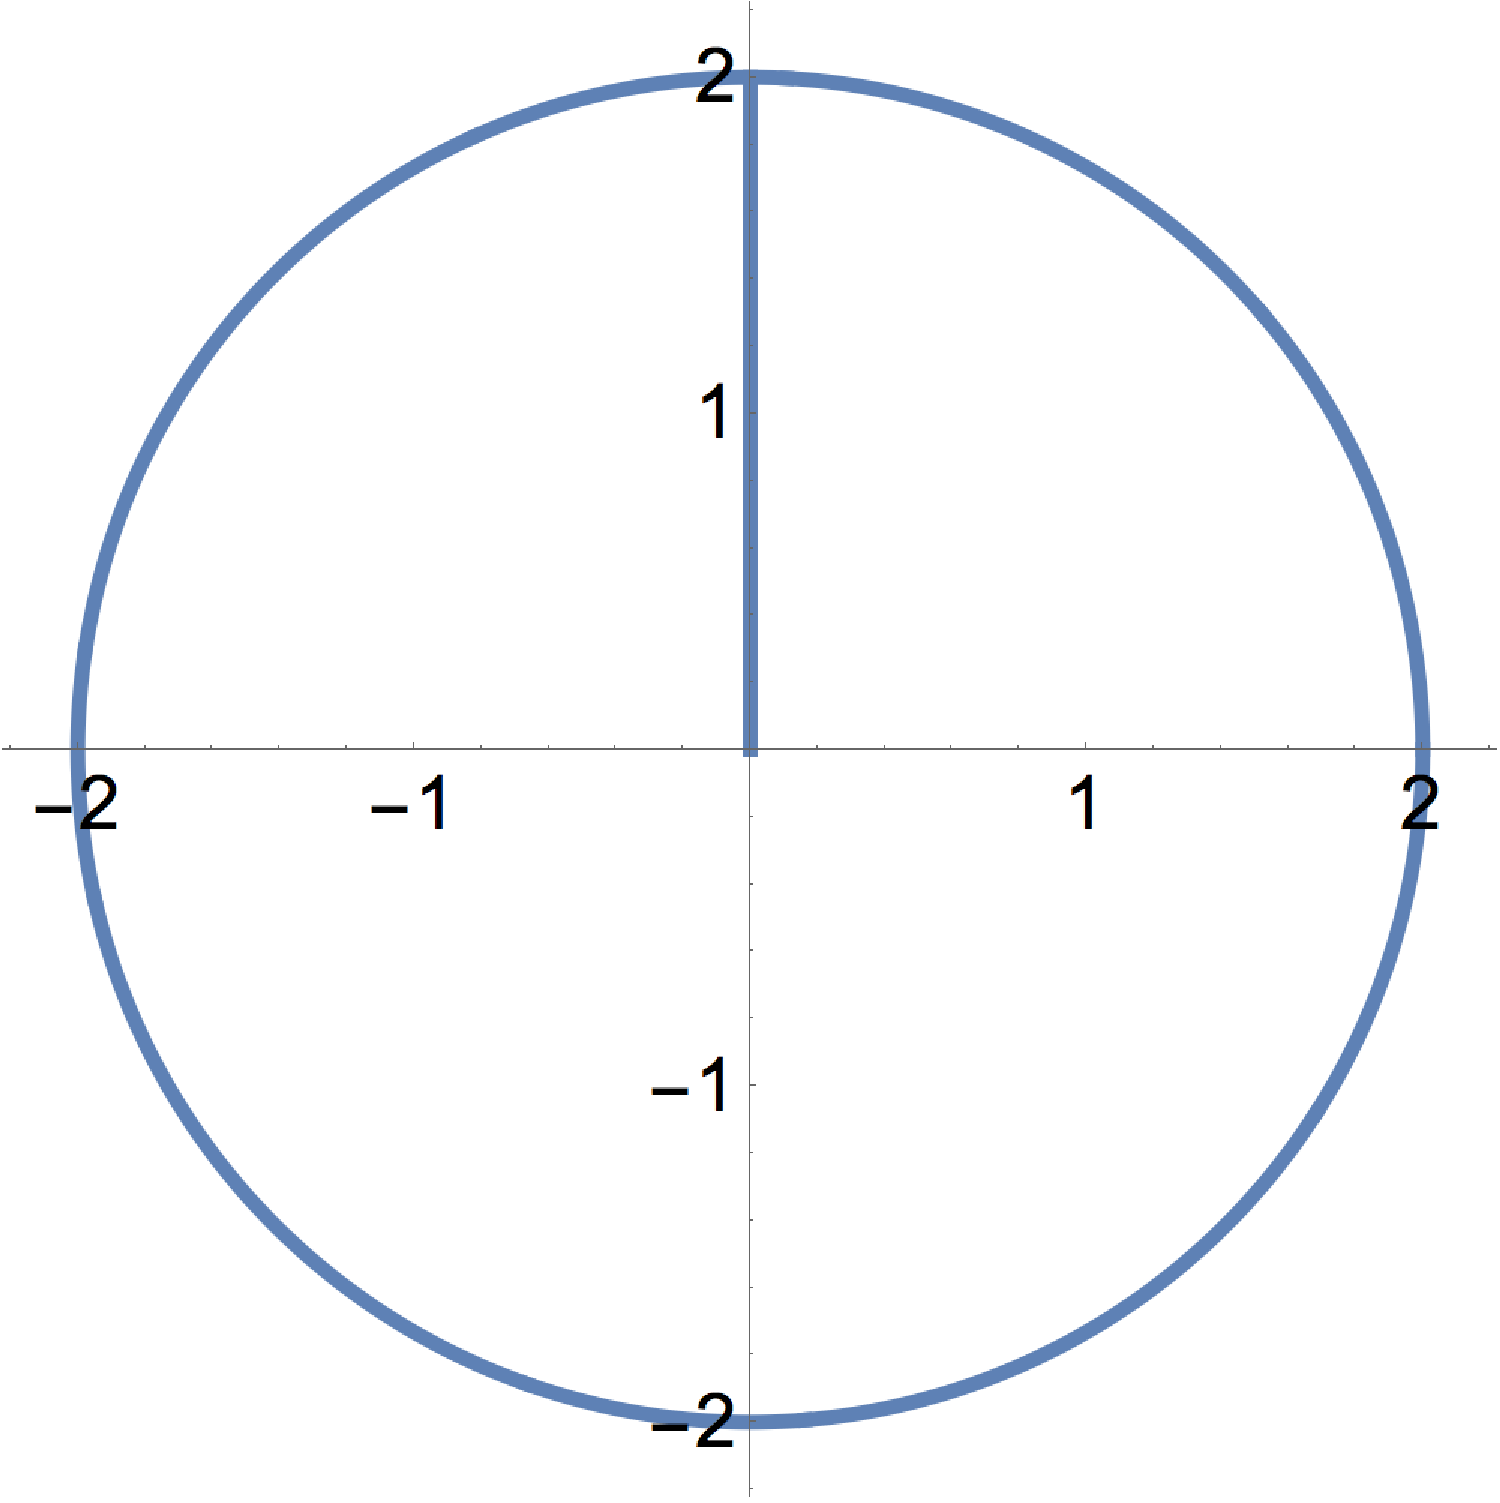
\includegraphics[scale=0.5]{circle.png}

\subsection*{Challenge}
Treating the x-axis as the real axis and the y-axis as the imaginary axis, arrange the equations below in the following order:

\begin{enumerate}
    \item A point moving round on a circle with radius 2 units and frequency 2 Hz
    \item A point moving round on a circle with radius 3 units and frequency 1 Hz
    \item A point moving round on a circle with radius 2 units and a period of 1 second
    \item A point moving round on a circle with radius 3 units and a period of 2 seconds
\end{enumerate}

Equations:

$\displaystyle A e^{2 \pi i k t}$ where $t$ is time in seconds and the values of $A$ and $k$ are as follows:

A: $A=2$, $k=2$ 

B: $A=3$, $k=1$

C: $A=3$, $k=0.5$

D: $A=2$, $k=1$

\subsection*{Solution}
\six{}

\hash{uu}{cb7845}

\timebox

% Convergence?
% Gibbs phenomena?


